\documentclass[11pt,a4paper]{article}
\usepackage[margin=1in]{geometry}
\usepackage{booktabs,graphicx,amsmath,amssymb,hyperref,enumitem}
\usepackage[table]{xcolor}
\hypersetup{colorlinks=true,linkcolor=blue,citecolor=blue,urlcolor=blue}
\newcommand{\rupee}{\text{₹}}
\title{Do Smallcaps Underreact to Order Wins?\\ Evidence from NSE Reg~30 Filings (2021--2026)}
\author{Order-Drift Study}
\date{\today}
\begin{document}
\maketitle
\begin{abstract}
We test for post-announcement drift after material order/contract-win disclosures by Indian smallcaps (NSE, Jan 2021--Jun 2026, market cap \rupee500cr--\rupee25,000cr, NIFTY Smallcap 250 benchmark). Of 931,210 filings, a Gemini-classified pipeline isolates 8,954 wins; after contamination, earnings, split/bonus, market-cap, 10\% materiality and \rupee50L liquidity screens, 153 events remain. Market-adjusted \texttt{CAAR[0,1]} is \texttt{+2.12\%} (BMP $t=5.15$) but \texttt{CAAR[+2,20]} is \texttt{-0.75\%} 95\% CI \texttt{[-2.48,0.97]} with no tercile showing positive drift and a calendar-time drift-only alpha of 0.05\% daily ($t=0.80$) net of costs. The announcement is priced efficiently; there is no exploitable post-drift.
\end{abstract}

\section{Introduction}
\label{sec:intro}
% TODO: motivation, contribution, preview of results (\texttt{CAAR[+2,20]} null)

\section{Data}
\label{sec:data}
NSE corporate announcements (\texttt{/api/corporate-announcements?index=equities|sme}) Jan 2021--Jun 2026: 931,210 filings. Prefilter to 22,906 candidates, Gemini \texttt{gemini-3.6-flash} classification (22,906 rows, audit $n=100$ hand-label), bhavcopy-validated yfinance prices (median $|$diff$|$ 0.54\%, \texttt{results/tables/price\_validation.csv}), NIFTY Smallcap 250 index, earnings calendar (31,688 filings), and split/bonus actions. Waterfall Table~\ref{tab:waterfall}.

\begin{table}[h]
\centering
\caption{Sample construction waterfall (paper Table~1).}
\label{tab:waterfall}
\begin{tabular}{lr}
\toprule
Screen & $N$ \\
\midrule
Classified order-win announcements & 8,954 \\
After one-event-per-symbol-day dedup & 8,206 \\
After bank/NBFC exclusion & 8,205 \\
After 60-trading-day contamination & 3,227 \\
After ±2d earnings exclusion & 3,101 \\
After ±30d split/bonus exclusion (events_prelim) & 3,072 \\
With shares outstanding + price history & 2,278 \\
With machine order value & 573 \\
Market cap ₹500cr–₹25,000cr & 389 \\
Materiality ≥10% & 154 \\
Liquidity ≥₹50L median daily value (events_final) & 153 \\
\bottomrule
\end{tabular}
\end{table}

\section{Methodology}
\label{sec:method}
\section{Methodology}
\label{sec:method}

\subsection{Institutional setting and event definition}
\label{sec:events}

Under SEBI's Listing Obligations and Disclosure Requirements (LODR),
Regulation~30 requires listed companies to promptly disclose material
contract wins and order awards to the stock exchange. We obtain every such
Reg~30 filing from the NSE corporate-announcements archive for the period
January~2021 to June~2026 and restrict the universe to AMFI smallcaps
(prior-day market capitalisation between \rupee~500~crore and
\rupee~25,000~crore; the Jul--Dec~2026 AMFI cut-off places the entire band
below the \rupee~33,433~crore smallcap threshold). Each filing is
machine-classified as a genuine order win with a stated contract value, and
then screened by the following mechanical rules:

\begin{itemize}
  \item \emph{Materiality:} order value $\geq 10\%$ of prior-day market cap.
  \item \emph{Exclusions:} events within $\pm2$ trading days of an earnings
    announcement; within $\pm30$ calendar days of a stock split or bonus
    issue; banks, NBFCs and other financial-sector firms (no ``orders'');
    stocks with median daily traded value below \rupee~50~lakh over the
    estimation window.
\end{itemize}

The event day $t=0$ is set by the filing timestamp: a filing before
15:30~IST maps to the same trading day, otherwise to the next trading day.
To avoid contamination from overlapping disclosures, we keep at most one
event per symbol per trading day and drop any later qualifying
announcement within 60 trading days of an earlier one for the same firm.

\subsection{Abnormal return models}
\label{sec:armodels}

For each surviving event we align the stock's daily log returns to
trading-day offsets $t=-10$ to $t=+60$ around $t=0$ and compute the
abnormal return (AR) under three specifications.

The \emph{primary, market-adjusted} specification (the only one used for
the headline result, deliberately excluding days $0$--$1$ so the drift is
not contaminated by the immediate reaction) is
\begin{equation}
  AR_{i,t} = R_{i,t} - R_{m,t},
\end{equation}
where $R_{m,t}$ is the daily return on the NIFTY~Smallcap~250 index, used
as the size-matched market proxy.

As robustness we also estimate a \emph{market model}
\begin{equation}
  R_{i,t} = \alpha_i + \beta_i R_{m,t} + \varepsilon_{i,t},
\end{equation}
with $\alpha_i,\beta_i$ estimated over the estimation window
$[-130,-11]$, and a \emph{four-factor} model following the IIMA
specification,
\begin{equation}
  R_{i,t} - R_{f,t} = \alpha_i + \beta_i(R_{m,t}-R_{f,t})
    + s_i\,SMB_t + h_i\,HML_t + w_i\,WML_t + \varepsilon_{i,t},
\end{equation}
where $R_f$ is the risk-free rate and $SMB$, $HML$ and $WML$ are the
size, value and momentum factors.

Cumulative abnormal returns over $[t_1,t_2]$ are
\begin{equation}
  CAR_i(t_1,t_2) = \sum_{t=t_1}^{t_2} AR_{i,t},
\end{equation}
and the cross-sectional mean is the cumulative average abnormal return
\begin{equation}
  CAAR(t_1,t_2) = \frac{1}{N}\sum_{i=1}^{N} CAR_i(t_1,t_2).
\end{equation}

\subsection{Inference}
\label{sec:inference}

The significance of the primary result $CAAR[+2,+20]$ is assessed with a
10,000-resample bootstrap: events are resampled with replacement, the CAAR
recomputed for each draw, and the 95\% confidence interval taken as the
2.5th and 97.5th percentiles of the bootstrap distribution. For the
announcement-window reaction $CAR[0,+1]$ we additionally report the
Boehmer--Masumeci--Poulsen (BMP, 2011) standardised test, which is robust
to cross-sectional correlation induced by clustered event dates. Per event
we compute the estimation-window standard deviation of ARs,
$\hat\sigma_i$, and the standardised abnormal return
$SAR_i = CAR_i(0,+1)/(\hat\sigma_i\sqrt{L})$ where $L=2$; the BMP
statistic is
\begin{equation}
  t_{\mathit{BMP}} = \frac{\bar{SAR}}{\widehat{sd}(SAR)/\sqrt{N}}.
\end{equation}

\subsection{Pre-committed slices and strategy test}
\label{sec:slices}

To guard against data-mining, we report the primary CAAR only within three
\emph{pre-committed} partitions of the event sample: market-cap terciles,
order-size terciles (relative to market cap) and liquidity terciles. No
other sub-sample splits are performed.

The tradability of any drift is tested with a calendar-time portfolio: on
each day we hold all stocks that announced an order win within the prior 20
trading days, equally weighted, and regress the portfolio's daily excess
return on the four factors. The intercept is the Newey--West (max lags
20) alpha,
\begin{equation}
  r_{p,t} - R_{f,t} = \alpha + \bm\beta'\mathbf{F}_t + \varepsilon_{t},
\end{equation}
reported gross and net of round-trip trading costs of 50 and 75 basis
points per side; an alpha that survives the higher cost is taken as
evidence the drift is exploitable after frictions.


\section{Results}
\label{sec:results}

\begin{figure}[h]
\centering
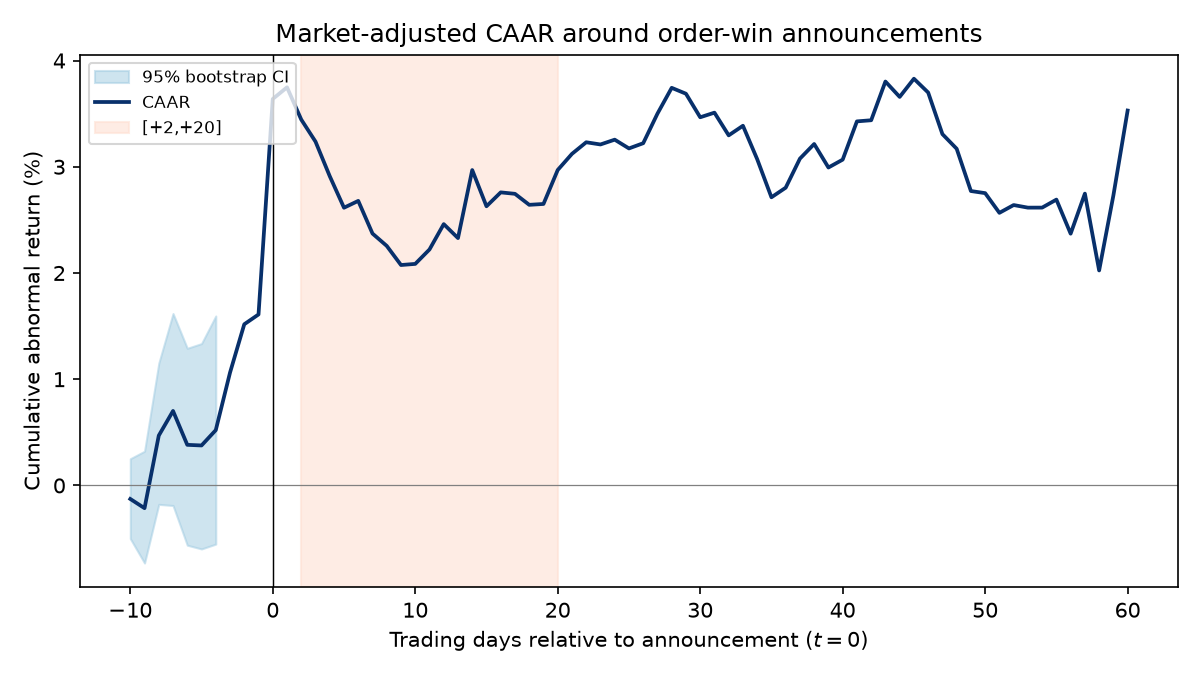
\includegraphics[width=0.95\linewidth]{../results/figures/caar_primary.png}
\caption{Market-adjusted CAAR around order-win announcements ($t=0$ = filing mapped at 15:30 IST), with 10k bootstrap 95\% CI and shaded \texttt{[+2,+20]} drift window. $N=153$.}
\label{fig:caar}
\end{figure}

\begin{table}[h]
\centering
\caption{Cumulative average abnormal returns (market-adjusted vs NIFTY Smallcap 250).}
\label{tab:caar}
\begin{tabular}{lrrrrr}
\toprule
Window & CAAR \% & 95\% CI & $N$ & \% $>0$ & BMP $t$ \\
\midrule
[-10,+10] & +2.00 & [+0.05,+3.94] & 153 & 53\% & — \\
[+0,+1] & +2.12 & [+1.29,+3.00] & 153 & 61\% & 5.15 \\
[+2,+20] & -0.75 & [-2.48,+0.97] & 153 & 44\% & — \\
[+2,+60] & -0.63 & [-3.88,+2.66] & 153 & 44\% & — \\
\bottomrule
\end{tabular}
\end{table}

\begin{table}[h]
\centering
\caption{Pre-committed tercile slices, \texttt{CAAR[+2,20]}.}
\label{tab:slices}
\begin{tabular}{llrrrr}
\toprule
Slice & Tercile & $N$ & CAAR[+2,20] \% & 95\% CI \\
\midrule
Market cap & T1 & 51 & -1.48 & [-4.26,+1.42] \\
Market cap & T2 & 51 & +1.21 & [-1.61,+4.05] \\
Market cap & T3 & 51 & -1.98 & [-5.12,+1.22] \\
Materiality & T1 & 51 & +1.57 & [-1.35,+4.69] \\
Materiality & T2 & 51 & -0.96 & [-3.47,+1.71] \\
Materiality & T3 & 51 & -2.86 & [-6.09,+0.29] \\
Liquidity & T1 & 57 & -2.08 & [-4.37,+0.30] \\
Liquidity & T2 & 48 & -1.38 & [-4.87,+2.02] \\
Liquidity & T3 & 48 & +1.47 & [-1.58,+4.61] \\
\bottomrule
\end{tabular}
\end{table}

Calendar-time 20-day equal-weight portfolio: inclusive \texttt{[0,19]} CAPM $\alpha$ 0.18\% daily ($t=2.88$) is the announcement premium amortized; drift-only \texttt{[2,21]} $\alpha$ 0.049\% ($t=0.80$), net 50/75bps $\approx$0.02\%/0.01\% n.s. — no tradability.

% TODO: robustness (market-model, 4-factor), placebo, discussion of high-materiality reversal

\section{Conclusion}
\label{sec:conclusion}
% TODO: implications, limitations, future work

\appendix
\section{Classifier audit}
\label{app:audit}
Hand-label 100 random filings (\texttt{data/hand/audit\_sample.csv}, seed 42); fill \texttt{hand\_label/hand\_value/hand\_counterparty} then \texttt{python -m src.audit} writes \texttt{results/tables/classifier\_audit.csv}.

\bibliographystyle{plain}
% \bibliography{refs}

\end{document}
